% !TeX root = ../thuthesis-example.tex
\chapter{bolt.SE 介绍}

本项目基于开源项目bolt.diy(以下简称bolt),在此基础上进行了多方面的优化和扩展。选择bolt作为基础平台的原因主要体现在以下几个方面:

\section{选择bolt的原因}

\begin{itemize}
    \item \textbf{开源与扩展性}: bolt作为一个开源平台,具备高度的扩展性和灵活性,便于根据项目的需求进行定制化开发,适应各种软件工程实践的要求。
    \item \textbf{多种大语言模型支持}: bolt支持多种大语言模型(LLM),如GPT-o3-mini、Claude 3.7 Sonnet等,且持续扩展对新模型的支持,这为代码生成提供了更多选择,极大地增强了系统的灵活性。
    \item \textbf{代码生成能力}: bolt具备出色的代码生成能力,尤其擅长理解和感知大规模复杂软件项目的上下文信息,在解析代码库和管理项目结构方面表现卓越。
    \item \textbf{WebContainer技术}: bolt使用WebContainer技术,使得代码能在浏览器中实时执行并预览,极大提升了开发的交互性和实时响应能力,便于开发者快速验证代码效果。
\end{itemize}

\section{系统整体流程}

bolt系统的流程图如图~\ref{fig:general_chat_sequence}所示。该图展示了从用户提交需求到最终生成并执行代码的完整流程。

\begin{figure}[ht]
  \centering
  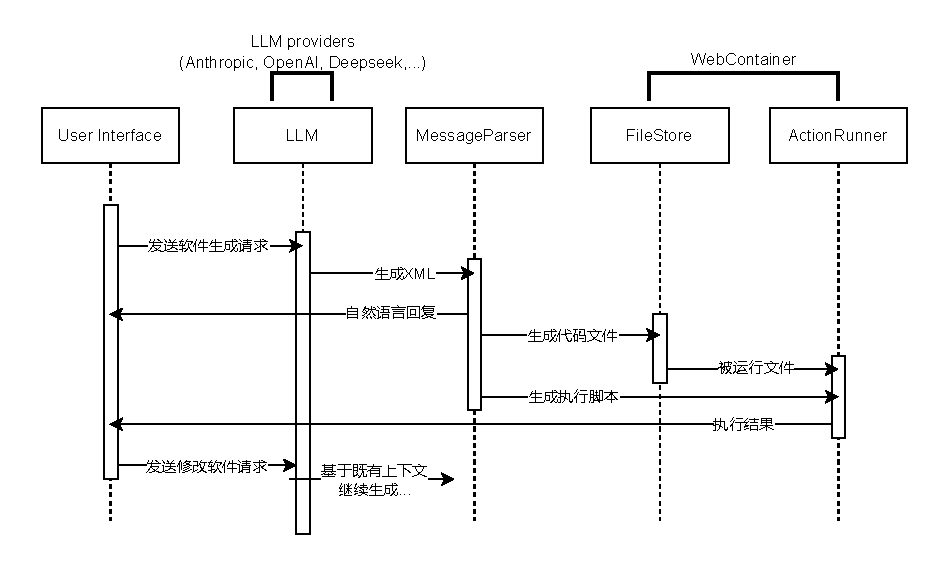
\includegraphics[width=1.0\linewidth]{general_chat_sequence.drawio.pdf}
  \caption{bolt.SE 代码生成时序图}
  \label{fig:general_chat_sequence}
\end{figure}

系统的整体流程包括以下几个关键步骤:
\begin{itemize}
    \item 用户通过UI界面输入需求,选择适当的大语言模型(LLM)。
    \item LLM生成自然语言响应,经过MessageParser模块解析为结构化XML格式。
    \item 生成的代码通过FileStore存储,并通过ActionRunner在WebContainer环境中执行。
    \item 执行结果通过ActionRunner反馈给用户,完成代码生成和执行过程。
\end{itemize}

其中,ActionRunner、FileStore 和 WebContainer 进行交互,WebContainer 提供了一个隔离、安全的运行环境,允许代码在浏览器中直接执行。WebContainer 的具体实现原理将在后续章节中详细介绍。

\section{UI与操作流程介绍}

bolt提供了一个直观易用的用户界面(UI),用户可以通过该界面方便地输入需求、选择模型、查看代码生成结果并进行进一步编辑。

\subsection{用户需求输入与模型选择}

用户在UI的左侧输入自然语言描述软件功能需求。bolt平台支持多种大语言模型(如OpenAI、Anthropic、DeepSeek等),用户可以根据需求选择适合的模型,以优化代码生成效果。

\subsection{代码生成与编辑}

根据用户输入的需求,bolt会自动调用选定的LLM生成代码,生成的代码会在在线IDE中展示。用户可以在IDE中进一步编辑、修改代码,并通过实时语法检查和错误提示功能及时发现问题。

\subsection{实时预览与调试}

bolt的WebContainer技术允许用户在浏览器中实时运行和预览生成的代码,开发者无需离开开发环境,即可直接验证代码的功能和效果。

\section{LLM介绍}

大语言模型(LLM)在本项目中的核心作用是生成代码并持续记忆上下文信息。以下分别介绍LLM在本项目中的应用及其优势。

\subsection{多LLM支持及其好处}

bolt支持多种LLM的接入,包括GPT-o3-mini、Claude 3.7 Sonnet等,未来还将进一步扩展对新模型的支持。具体而言,bolt内部已对多种LLM提供商的API进行了封装,用户只需向各平台申请API Key,并配置在系统中,即可使用对应的模型。
这一多模型支持的优势在于:
\begin{itemize}
    \item 用户可以根据具体的项目需求,选择最适合的模型,优化代码生成效果。
    \item 通过灵活切换模型,能够适应不同的代码生成任务,如前端开发、后端开发等,提供更好的定制化能力。
    \item 多模型支持减少对单一模型的依赖,避免出现由于某个模型的缺陷或更新导致的不可用情况。
\end{itemize}

\subsection{大语言模型的超长文本处理能力}

传统的代码生成工具,如GitHub Copilot、Cursor和DeepSeek等,通常在生成代码时只关注当前输入的单一上下文片段或局限于当前编辑区域附近的上下文。这导致当代码库规模增大时,生成的代码可能缺乏一致性,或忽略已有代码库的风格和约定。

而在bolt平台中,由于所有的代码生成过程本质上都表现为用户与大语言模型之间一来一往的交互对话,因此,整个项目的代码库实际上就是一系列高度结构化的“对话记录”。利用LLM的超长文本处理能力,bolt能够将这些累积的对话历史完整地纳入模型的记忆上下文。这种独特的设计使LLM不仅能基于当前用户输入生成代码,还能够回顾并记忆历史生成的代码片段、开发者的设计决策以及代码库整体的架构约定。

\section{MessageParser}

MessageParser是系统中的一个关键模块,负责将大语言模型(LLM)生成的自然语言响应解析为结构化的数据格式,通常是XML格式。该XML格式不仅包含生成的代码,还包括后续的操作步骤、文件路径等信息,能够高效地支持后续的代码生成和执行等任务。下面以一个创建JavaScript函数的例子来详细说明XML结构的组成及其各标签的功能。

\subsection{Prompt定义的XML结构}

为了便于MessageParser解析和处理LLM的输出,我们设计了一个特定的XML结构。该结构能够清晰地表达每一步生成的代码和执行的操作。以下是一个例子,展示了如何通过XML结构描述一个创建JavaScript函数的过程:

\begin{lstlisting}[breaklines=true,basicstyle=\ttfamily\small]
<example>
  <user_query>Can you help me create a JavaScript function to calculate the factorial of a number?</user_query>
  <assistant_response>
    Certainly, I can help you create a JavaScript function to calculate the factorial of a number.

    <boltArtifact id="factorial-function" title="JavaScript Factorial Function">
      <boltAction type="file" filePath="index.js">
        function factorial(n) {
          return n <= 1 ? 1 : n * factorial(n - 1);
        }
      </boltAction>

      <boltAction type="shell">node index.js</boltAction>
    </boltArtifact>
  </assistant_response>
</example>
\end{lstlisting}

\subsubsection{XML标签说明}

这个XML结构中,主要涉及以下几个标签和子标签:

\begin{itemize}
    \item \textbf{\textless user\_query\textgreater}: 该标签包含用户输入的自然语言查询。在本例中,用户请求创建一个计算阶乘的JavaScript函数。
    
    \item \textbf{\textless assistant\_response\textgreater}: 该标签包含LLM的自然语言响应。它不仅包括对用户查询的文本回复,还包括后续的操作步骤,通常是通过`boltArtifact`和`boltAction`来描述代码生成和执行的过程。
    
    \item \textbf{\textless boltArtifact\textgreater}: 这是一个容器标签,用于表示一个生成的代码单元或"工件"。在本例中,`boltArtifact`表示生成的JavaScript阶乘函数。它具有两个重要的属性:
    \begin{itemize}
        \item \textbf{id}: 唯一标识符,用于引用和管理生成的代码单元。
        \item \textbf{title}: 标题或描述,帮助用户理解该工件的内容。在此例中,标题是"JavaScript Factorial Function"。
    \end{itemize}
    
    \item \textbf{\textless boltAction\textgreater}: 这是描述具体操作的标签,它包含了代码生成、文件操作和执行指令等步骤。每个`boltAction`代表一个单独的操作,可以是文件生成、命令执行等。在本例中,`boltAction`有两种类型:
    \begin{itemize}
        \item \textbf{type="file"}: 表示这是一个文件操作,文件内容就是生成的JavaScript函数。`filePath`属性指定了文件的路径,这里是`index.js`,它是包含阶乘函数的文件。
        \item \textbf{type="shell"}: 表示这是一个命令行操作,`boltAction`标签中的内容是一个shell命令。在本例中,命令是`node index.js`,表示在命令行中运行生成的JavaScript文件。
    \end{itemize}
\end{itemize}

\subsubsection{如何处理XML结构}

在实际应用中,MessageParser会根据LLM的输出将自然语言响应转换为这种XML结构。每个操作步骤都会被封装成`boltAction`,而所有的操作步骤将组成一个`boltArtifact`,最终这些`boltArtifact`构成了完整的代码生成流程。

1. 用户的查询会被传递给LLM,LLM解析查询并生成自然语言响应(如上例中的JavaScript代码)。
2. MessageParser接收LLM的响应,并将其转换为结构化的XML数据,其中包含了生成的代码(如`factorial`函数)及相关操作(如创建文件和执行代码)。
3. 系统根据这些`boltArtifact`和`boltAction`执行相应的操作,如创建文件、执行命令等。

\subsection{结构化数据的优势}

通过将LLM生成的自然语言响应转化为结构化的XML格式,MessageParser能够高效地将生成的代码和操作步骤传递给后续模块,如FileStore和ActionRunner。这种结构化方式使得系统能够:
\begin{itemize}
    \item 高效地管理和执行多个代码生成和执行任务。
    \item 便于扩展和定制化,可以根据具体需求调整`boltAction`的类型和操作。
    \item 提供清晰的反馈和调试信息,帮助开发者快速定位问题。
\end{itemize}

总之,XML格式不仅是LLM与系统之间的桥梁,还能够促进后续操作的自动化和可管理性,从而提升整个系统的效率和可扩展性。

\section{WebContainer简介}

WebContainer 是由 StackBlitz 开发的基于 WebAssembly 的微型操作系统,旨在在浏览器中原生运行 Node.js 环境。它通过将 Node.js 编译为 WebAssembly(WASM),使开发者能够在浏览器中直接执行服务器端代码,如运行 Node.js 服务器、安装 npm 包等。 

\subsection{实现原理}

WebContainer 的核心在于利用 WebAssembly 技术,将 Node.js 及相关工具链编译为可在浏览器中运行的格式。具体而言,它在浏览器中模拟了一个完整的操作系统环境,包括文件系统和进程管理等功能。这使得开发者可以在浏览器中执行诸如 \texttt{npm install}、\texttt{node index.js} 等命令,实现完整的开发工作流程。 

\subsection{在 bolt 系统中的应用}

在 bolt 系统中,WebContainer 被用于提供一个安全、隔离的运行环境,以支持代码的生成和执行:

\begin{enumerate}

    \item 代码存储:生成的代码通过 FileStore 模块存储在 WebContainer 的虚拟文件系统中,确保代码资产的安全管理和版本控制。

    \item 代码执行:ActionRunner 模块从 FileStore 获取代码,并在 WebContainer 环境中执行。由于 WebContainer 提供了完整的 Node.js 运行时,代码可以在其中被直接运行。

    \item 结果反馈:执行结果通过 ActionRunner 返回给用户,并进行渲染。
\end{enumerate}

通过上述流程,bolt 系统利用 WebContainer 的能力,实现了在浏览器中直接进行代码的生成、存储、执行和反馈,使使用者能够实时看到代码的执行结果,极大地提升了开发效率和用户体验。 

\section{改进}

% TODO
本项目在bolt的基础上,进行了以下改进:

